\documentclass[wide,a4paper,titlepage,12pt] {article}
\usepackage{polski}
\usepackage[UTF8]{inputenc}
\usepackage{listings}
\usepackage{slashbox}
\usepackage[table]{xcolor}
\usepackage{graphicx,pdflscape}
\usepackage{placeins}


\title{Grafika komputerowa}
\author{Jacek Wieczorek (181043)}

% Title page layout (fold)
\makeatletter
\renewcommand{\maketitle}{
\begin{titlepage}
  \begin{center}
    \vspace*{3cm}
    \LARGE \@title \par
    \vspace{2cm}
    \textit{\small Autor:}\par
    \normalsize \@author\par \normalsize
    \vspace{3cm}
    \textit{\small Prowadzący:}\par
    Dr inż. Tomasz Kapłon \par
    \vspace{2cm}
    Wydział Elektroniki\\ III rok\\ Pn TP 08.15 - 11.00\par
    \vspace{4cm}
    \small \@date
  \end{center}
\end{titlepage}
}
\makeatother
% Title page layout (end)



\begin{document}
\maketitle
  \section{Cel laboratorium}
\paragraph{}
Celem ćwiczenia jest  ilustracja możliwości oświetlania obiektów na scenach $3-D$  z wykorzystaniem biblioteki $OpenGL$ z rozszerzeniem $GLUT$, sterowania oświetleniem oraz budowy własnego modelu oświetlenia.

\section{Zadanie 1}
\paragraph{}
Pierwsze zadanie polegało na oświetleniu jednym żródłem śiwatła obracającego się jajka, stworzonego podczas laboratorium drugiego. W celu poprawnego oświetlenia jajka, korzystając z modelu Phong'a, należy wyliczyć wektor normalny z następujących zależności : \\ \\
Powierzchnia jajka opisana została równaniem : \\
 \begin{figure}[htbp]
      \begin{center}
       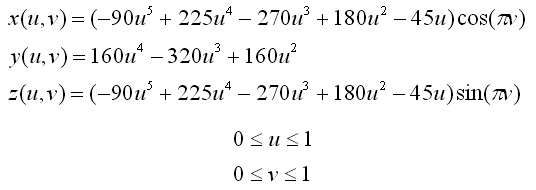
\includegraphics[width=\textwidth]{wzor_2.jpg}
	\label{fig5}
      \end{center}
    \end{figure}
\newpage
Wektor normalny można znaleźć za pomocą nastepujących równań :\\
 \begin{figure}[htbp]
      \begin{center}
       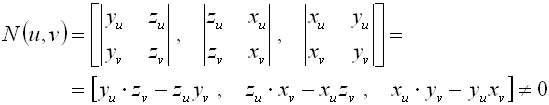
\includegraphics[width=\textwidth]{wzor_0.jpg}
	\label{fig5}
      \end{center}
    \end{figure}

Gdzie : 
 \begin{figure}[htbp]
      \begin{center}
       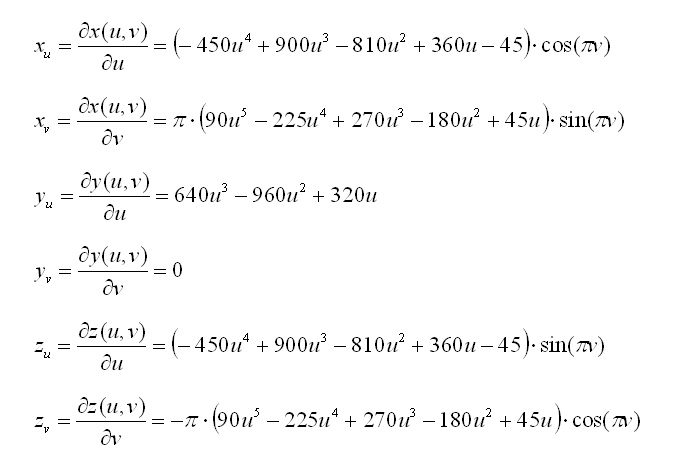
\includegraphics[width=\textwidth]{wzor.jpg}
	\label{fig5}
      \end{center}
    \end{figure} \newpage
\subsection{Funkcje programu :}
\subsubsection{Obliczanie współrzędnych powierzchni jajka i wektora normalnego}
\lstset{ %
    language=c++,                % choose the language of the code
    basicstyle=\scriptsize,       % the size of the fonts that are used for the code
    numbers=left,                   % where to put the line-numbers
    numberstyle=\scriptsize,      % the size of the fonts that are used for the line-numbers
    stepnumber=10,                   % the step between two line-numbers. If it's 1 each line 
                                    % will be numbered
    numbersep=9pt,                  % how far the line-numbers are from the code
    % backgroundcolor=\color{white},  % choose the background color. You must add \usepackage{color}
    showspaces=false,               % show spaces adding particular underscores
    showstringspaces=false,         % underline spaces within strings
    showtabs=false,                 % show tabs within strings adding particular underscores
    % frame=single,                 % adds a frame around the code
    % tabsize=2,                  % sets default tabsize to 2 spaces
    % captionpos=b,                   % sets the caption-position to bottom
    breaklines=true,                % sets automatic line breaking
    % breakatwhitespace=false,        % sets if automatic breaks should only happen at whitespace
    % title=\lstname,                 % show the filename of files included with \lstinputlisting;
                                    % also try caption instead of title
    % escapeinside={\%*}{*)},         % if you want to add a comment within your code
    % morekeywords={*,...}            % if you want to add more keywords to the set
    }
    \lstinputlisting{z1.cpp}
\subsubsection{Ustawienie parametrów materiału i źródła światła}
\lstset{ %
    language=c++,                % choose the language of the code
    basicstyle=\scriptsize,       % the size of the fonts that are used for the code
    numbers=left,                   % where to put the line-numbers
    numberstyle=\scriptsize,      % the size of the fonts that are used for the line-numbers
    stepnumber=10,                   % the step between two line-numbers. If it's 1 each line 
                                    % will be numbered
    numbersep=9pt,                  % how far the line-numbers are from the code
    % backgroundcolor=\color{white},  % choose the background color. You must add \usepackage{color}
    showspaces=false,               % show spaces adding particular underscores
    showstringspaces=false,         % underline spaces within strings
    showtabs=false,                 % show tabs within strings adding particular underscores
    % frame=single,                 % adds a frame around the code
    % tabsize=2,                  % sets default tabsize to 2 spaces
    % captionpos=b,                   % sets the caption-position to bottom
    breaklines=true,                % sets automatic line breaking
    % breakatwhitespace=false,        % sets if automatic breaks should only happen at whitespace
    % title=\lstname,                 % show the filename of files included with \lstinputlisting;
                                    % also try caption instead of title
    % escapeinside={\%*}{*)},         % if you want to add a comment within your code
    % morekeywords={*,...}            % if you want to add more keywords to the set
    }
    \lstinputlisting{z2.cpp}
\subsubsection{Rysowanie jajka}
\lstset{ %
    language=c++,                % choose the language of the code
    basicstyle=\scriptsize,       % the size of the fonts that are used for the code
    numbers=left,                   % where to put the line-numbers
    numberstyle=\scriptsize,      % the size of the fonts that are used for the line-numbers
    stepnumber=10,                   % the step between two line-numbers. If it's 1 each line 
                                    % will be numbered
    numbersep=9pt,                  % how far the line-numbers are from the code
    % backgroundcolor=\color{white},  % choose the background color. You must add \usepackage{color}
    showspaces=false,               % show spaces adding particular underscores
    showstringspaces=false,         % underline spaces within strings
    showtabs=false,                 % show tabs within strings adding particular underscores
    % frame=single,                 % adds a frame around the code
    % tabsize=2,                  % sets default tabsize to 2 spaces
    % captionpos=b,                   % sets the caption-position to bottom
    breaklines=true,                % sets automatic line breaking
    % breakatwhitespace=false,        % sets if automatic breaks should only happen at whitespace
    % title=\lstname,                 % show the filename of files included with \lstinputlisting;
                                    % also try caption instead of title
    % escapeinside={\%*}{*)},         % if you want to add a comment within your code
    % morekeywords={*,...}            % if you want to add more keywords to the set
    }
    \lstinputlisting{z3.cpp} \newpage
\subsection{Przykładowy wynik}
 \begin{figure}[htbp]
      \begin{center}
       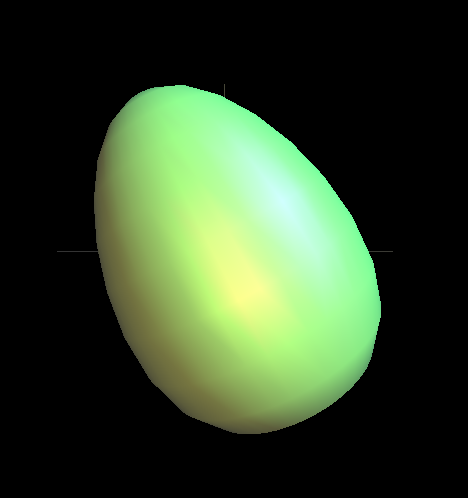
\includegraphics[width=\textwidth]{jajko1.PNG}
	\label{fig5}
      \end{center}
    \end{figure}
\newpage
\section{Zadanie 2}
\paragraph{}
Zadanie 2 polegało na dodaniu kolejnego źródła światła i możliwości sterowania nimi za pomocą myszki poprze zmianę kątów azymutu i elewacji.
\subsection{Kod programu}
\subsubsection{Dodanie drugiego źródła światła}
\lstset{ %
    language=c++,                % choose the language of the code
    basicstyle=\scriptsize,       % the size of the fonts that are used for the code
    numbers=left,                   % where to put the line-numbers
    numberstyle=\scriptsize,      % the size of the fonts that are used for the line-numbers
    stepnumber=10,                   % the step between two line-numbers. If it's 1 each line 
                                    % will be numbered
    numbersep=9pt,                  % how far the line-numbers are from the code
    % backgroundcolor=\color{white},  % choose the background color. You must add \usepackage{color}
    showspaces=false,               % show spaces adding particular underscores
    showstringspaces=false,         % underline spaces within strings
    showtabs=false,                 % show tabs within strings adding particular underscores
    % frame=single,                 % adds a frame around the code
    % tabsize=2,                  % sets default tabsize to 2 spaces
    % captionpos=b,                   % sets the caption-position to bottom
    breaklines=true,                % sets automatic line breaking
    % breakatwhitespace=false,        % sets if automatic breaks should only happen at whitespace
    % title=\lstname,                 % show the filename of files included with \lstinputlisting;
                                    % also try caption instead of title
    % escapeinside={\%*}{*)},         % if you want to add a comment within your code
    % morekeywords={*,...}            % if you want to add more keywords to the set
    }
    \lstinputlisting{z4.cpp} \newpage
\subsubsection{Sterowanie oświetleniem}
\lstset{ %
    language=c++,                % choose the language of the code
    basicstyle=\scriptsize,       % the size of the fonts that are used for the code
    numbers=left,                   % where to put the line-numbers
    numberstyle=\scriptsize,      % the size of the fonts that are used for the line-numbers
    stepnumber=10,                   % the step between two line-numbers. If it's 1 each line 
                                    % will be numbered
    numbersep=9pt,                  % how far the line-numbers are from the code
    % backgroundcolor=\color{white},  % choose the background color. You must add \usepackage{color}
    showspaces=false,               % show spaces adding particular underscores
    showstringspaces=false,         % underline spaces within strings
    showtabs=false,                 % show tabs within strings adding particular underscores
    % frame=single,                 % adds a frame around the code
    % tabsize=2,                  % sets default tabsize to 2 spaces
    % captionpos=b,                   % sets the caption-position to bottom
    breaklines=true,                % sets automatic line breaking
    % breakatwhitespace=false,        % sets if automatic breaks should only happen at whitespace
    % title=\lstname,                 % show the filename of files included with \lstinputlisting;
                                    % also try caption instead of title
    % escapeinside={\%*}{*)},         % if you want to add a comment within your code
    % morekeywords={*,...}            % if you want to add more keywords to the set
    }
    \lstinputlisting{z5.cpp} 
\newpage
\subsection{Przykładowy wynik}
 \begin{figure}[htbp]
      \begin{center}
       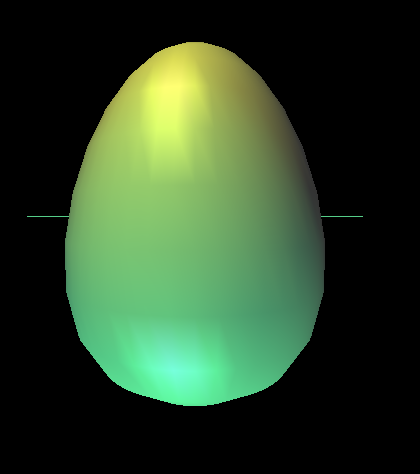
\includegraphics[width=\textwidth]{jajko2.PNG}
      \end{center}
    \end{figure}
\newpage
\section{Wnioski}
\paragraph{}
Oświetlanie obiektu w OpenGL za pomocą modelu Phong'a nie jest skomplikowanym zadaniem. Problematyczne okazuje się wyliczenie wektorów normalnych powierzchni obiektu nie wchodzącego w skład biblioteki. Te utrudnienia nie występowały przy generowaniu oświetlenia dla czajniczka, będącego częścią biblioteki OpenGL i GLUT.

\end{document}